\documentclass[a4paper, twoside, english]{article}

\usepackage{amsmath}
\usepackage{amsfonts}
\usepackage{ihci}
\usepackage{graphicx}
\usepackage{subfig}

\newcommand\tab[1][0.4cm]{\hspace*{#1}}
\setlength{\parindent}{0pt}

\graphicspath{{./figures/}}

\title{Exercise 2 \\ 3D Computer Vision}  % Replace "Template Report" with Exercise 1, Exercise 2, etc
\author{Shoaib Ahmed Siddiqui}                       % Replace with your names
\date{01.12.2017}                              % Replace with current date

\begin{document}

\maketitle

\section{Theory}

\underline{\textbf{Properties of Rotation Matrices}}

\textbf{1. Show that $U^{T} = U^{-1}$.}

The most generic form of rotation matrices in 3D can be defined as:

\abovedisplayskip
\begin{equation*}
\begin{align*}
 R_z (\theta) &= \left[
 \begin{array}{ccc}
  cos(\theta) & -sin(\theta) & 0 \\
  sin(\theta) & cos(\theta) & 0 \\
  0 & 0 & 1
 \end{array}
 \right] \\
 R_y (\psi) &= \left[
 \begin{array}{ccc}
  cos(\psi) & 0 & sin(\psi) \\
  0 & 1 & 0 \\
  -sin(\psi) & 0 & cos(\psi)
 \end{array}
 \right] \\
 R_x (\phi) &= \left[
 \begin{array}{ccc}
  1 & 0 & 0 \\
  0 & cos(\phi) & -sin(\phi) \\
  0 & sin(\phi) & cos(\phi)
 \end{array}
 \right]
 \label{eq:allRotationMatrices}
\end{align*}
\end{equation*}

Let us consider just one of the rotation matrix $R_z (\theta)$ along with its transpose:

\begin{align*}
 R_z (\theta) = \left[
 \begin{array}{ccc}
  cos(\theta) & -sin(\theta) & 0 \\
  sin(\theta) & cos(\theta) & 0 \\
  0 & 0 & 1
 \end{array}
 \right] \\
 R_z (\theta)^{T} = \left[
 \begin{array}{ccc}
  cos(\theta) & sin(\theta) & 0 \\
  -sin(\theta) & cos(\theta) & 0 \\
  0 & 0 & 1
 \end{array}
 \right] 
 \label{eq:rotationMatricesForZAxis}
\end{align*}

Given these two matrices, we can directly multiply them.

\begin{equation}
 R_z (\theta) * R_z (\theta)^{T} = \left[
 \begin{array}{ccc}
  cos^2(\theta) + sin^2(\theta) & cos(\theta)sin(\theta) - sin(\theta)cos(\theta) & 0 \\
  sin(\theta)cos(\theta) - cos(\theta)sin(\theta) & sin^2(\theta) + cos^2(\theta) & 0 \\
  0 & 0 & 1
 \end{array}
 \right]
 \label{eq:rotationMatricesMultiplication}
\end{equation}

\begin{equation}
 \begin{aligned}
  sin^2(\theta) + cos^2(\theta) &= 1 \\
          sin(\alpha - \beta) &= sin(\alpha)cos(\beta) - cos(\alpha)sin(\beta)
 \end{aligned}
 \label{eq:trigIdentities}
\end{equation}

Using the famous trigonometric identities given in Eq.~\ref{eq:trigIdentities}, Eq.~\ref{eq:rotationMatricesMultiplication} can be written as:

\begin{equation*}
\begin{align*}
 R_z (\theta) * R_z (\theta)^{T} &= \left[
 \begin{array}{ccc}
  1 & sin(\theta - \theta) & 0 \\
  sin(\theta - \theta) & 1 & 0 \\
  0 & 0 & 1
 \end{array}
 \right] \\
 R_z (\theta) * R_z (\theta)^{T} &= \left[
 \begin{array}{ccc}
  1 & sin(0) & 0 \\
  sin(0) & 1 & 0 \\
  0 & 0 & 1
 \end{array}
 \right] \\
 R_z (\theta) * R_z (\theta)^{T} &= \left[
 \begin{array}{ccc}
  1 & 0 & 0 \\
  0 & 1 & 0 \\
  0 & 0 & 1
 \end{array}
 \right]
 \label{eq:rotationMatricesMultiplication2}
\end{align*}
\end{equation*}

The same can be shown for $R_x (\psi)$ and $R_y (\phi)$. \\

\textbf{2. Geometric interpretation of the determinent of a square $3\times3$ matrix A.}

Matrix A performs a linear transformation of the input vector $\textbf{x}$ as given in Eq~\ref{eq:linearTransform}. 
\begin{equation}
 A\textbf{x} = \textbf{b}
 \label{eq:linearTransform}
\end{equation}

The determinent of matrix A represents the volume distortion experienced by the region defined by vector \textbf{x}. The sign of the determinent represents if the transformation will preserve the orientation.
Let us consider the input vector $\textbf{x}$ to be of unit area in the standard basis. After the linear transformation through the matrix A, the vector $\textbf{x}$ will change its area to $|(det A)|$. 
Since for rotations, translations, and other linear transformations, we would like to preserve the scale of the input, therefore, we take matrices with unit determinent. This leads to input transformation without any change in scale ~\cite{determinent}.

\bigbreak
\underline{\textbf{Transformation Chain}}

The step step in the transformation chain is to transform the point from the world coordinate system to the camera coordinate system. We consider two types of transformations between the coordinate frames. These two transformations are rotation and translation.
Let us consider a point in 3D defined by $\textbf{x}$ in the world coordinate system. Then, the projection of $\textbf{x}$ in the camera coordinate system can be denoted via $\tilde{\textbf{x}}$ and can be computed as:

\begin{equation}
 \tilde{\textbf{x}} = R\textbf{x} + \textbf{t}
 \label{eq:worldToCameraSample}
\end{equation}

In Eq.~\ref{eq:worldToCameraSample}, $R$ is the rotation matrix while $\textbf{t}$ is the translation vector. The projection from 3D to 2D can be achieved by throwing out the last coordinate, i.e. $(x,y,z) \to (f'x/z, f'y/z)$. 
Division by $z$ makes this transformation non-linear. This transformation can be converted to a linear transformation via adding another coordinate to the vector making it homogeneous i.e. $(x,y,w) \to (x/w, y/w)$ for 2D points and $(x,y,z,w) \to (x/w, y/w, z/w)$ for 3D points. The final coordinate represents the scale, hence, homogeneous coordinates are scale invariant.
Hence, the transformation from world coordinate system to camera coordinate system can be rewritten as:

\begin{equation*}
 \left[
 \begin{array}{c}
  \tilde{x} \\
  \tilde{y} \\
  \tilde{z} \\
  1
 \end{array}
 \right] =
 \left[
 \begin{array}{cc}
  R & \textbf{t} \\
  0_{3}^{T} & 1  
 \end{array}
 \right]
 \left[
 \begin{array}{c}
  x \\
  y \\
  z \\
  1
 \end{array}
 \right]
 \label{eq:worldToCamera}
\end{equation*}

In this linear transformation, $R$ and $T$ are extrinsic parameters of the camera. The point $\tilde{\textbf{x}}$ in camera coordinate system has to now go through the perspective transformation and final projection onto the image plane. 
This transformation is captured by the intrinsic camera parameters $K$. Let $\alpha_{x}, \alpha_{y}$ be the focal length of the camera in pixels, $(x_0, y_0)$ be the coordinates of the image center in pixels and $s$ be the skew parameter, then the final transformation mapping the camera coordinates to image plane can be written as:

\begin{equation*}
 \left[
 \begin{array}{c}
  u' \\
  v' \\
  w' \\
 \end{array}
 \right] =
 \left[
 \begin{array}{cccc}
  \alpha_{x} & s & x_{0} & 0 \\
  0 & \alpha_{y} & y_{0} & 0 \\
  0 & 0 & 1 & 0
 \end{array}
 \right]
 \left[
 \begin{array}{c}
  \tilde{x} \\
  \tilde{y} \\
  \tilde{z} \\
  1
 \end{array}
 \right]
 \label{eq:perspectiveProjection}
\end{equation*}

The 2D homogeneous coordinates can be converted to 2D point via normalization of the scale i.e. $(u',v',w') \to (u'/w', v'/w')$. The normalized point $(u'/w', v'/w')$ can be denoted as $(x_{pix}, y_{pix})$ specifies the location of the point in the image plane.

\section{Implementation}

Fig.~\ref{fig:pointProjection} visualizes the output of the main.py script which transforms the points provided in the 3D world coordinate system to the image coordinates. 
Fig.~\ref{fig:pointProjection} (left) is the output without correction of radial distortion present in the camera. It is evident from the image that the visualized points are not perfectly aligned with the corners present in the checkerboard.
Once the radial distortion is catered through the provided distortion parameters, the points got perfectly aligned with the corners in the checkerboard which is visualized in Fig.~\ref{fig:pointProjection} (right).

\begin{figure}[h]
 \centerline
 {
  \subfloat[]{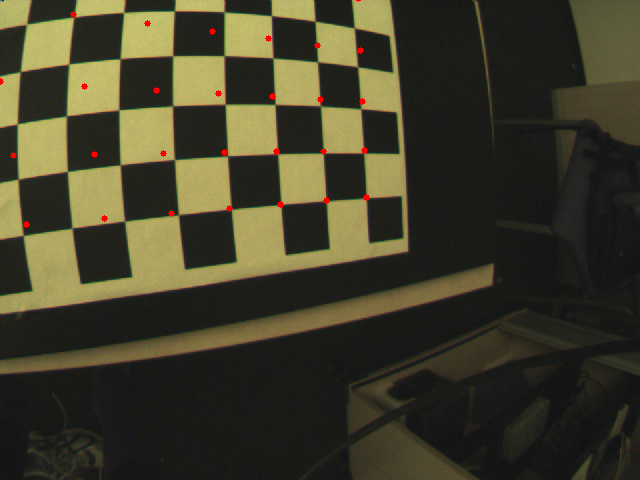
\includegraphics[width=0.35\textwidth]{out.png}}
  \qquad
  \subfloat[]{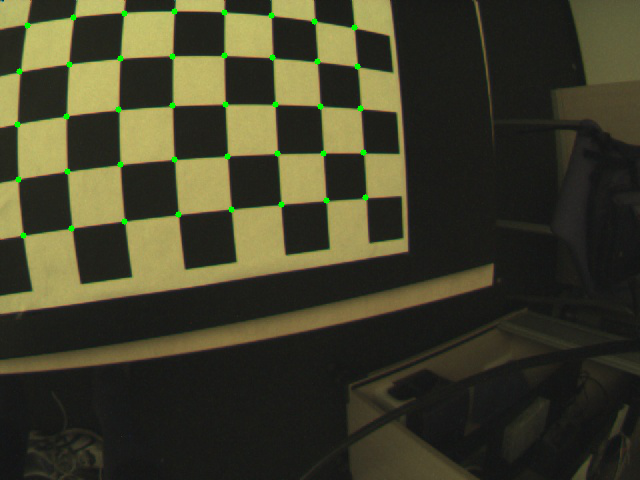
\includegraphics[width=0.35\textwidth]{out-radial.png}}
 }
 \caption[3D Point Projection]{(a) Without correction of radial distortion. (b) With correction of radial distortion.}
 \label{fig:pointProjection}
\end{figure}

\bibliographystyle{plain}
\bibliography{bibliography.bib}
\end{document}